% Options for packages loaded elsewhere
\PassOptionsToPackage{unicode}{hyperref}
\PassOptionsToPackage{hyphens}{url}
%
\documentclass[
  10pt,
  ignorenonframetext,
]{beamer}
\usepackage{pgfpages}
\setbeamertemplate{caption}[numbered]
\setbeamertemplate{caption label separator}{: }
\setbeamercolor{caption name}{fg=normal text.fg}
\beamertemplatenavigationsymbolsempty
% Prevent slide breaks in the middle of a paragraph
\widowpenalties 1 10000
\raggedbottom
\setbeamertemplate{part page}{
  \centering
  \begin{beamercolorbox}[sep=16pt,center]{part title}
    \usebeamerfont{part title}\insertpart\par
  \end{beamercolorbox}
}
\setbeamertemplate{section page}{
  \centering
  \begin{beamercolorbox}[sep=12pt,center]{part title}
    \usebeamerfont{section title}\insertsection\par
  \end{beamercolorbox}
}
\setbeamertemplate{subsection page}{
  \centering
  \begin{beamercolorbox}[sep=8pt,center]{part title}
    \usebeamerfont{subsection title}\insertsubsection\par
  \end{beamercolorbox}
}
\AtBeginPart{
  \frame{\partpage}
}
\AtBeginSection{
  \ifbibliography
  \else
    \frame{\sectionpage}
  \fi
}
\AtBeginSubsection{
  \frame{\subsectionpage}
}
\usepackage{lmodern}
\usepackage{amssymb,amsmath}
\usepackage{ifxetex,ifluatex}
\ifnum 0\ifxetex 1\fi\ifluatex 1\fi=0 % if pdftex
  \usepackage[T1]{fontenc}
  \usepackage[utf8]{inputenc}
  \usepackage{textcomp} % provide euro and other symbols
\else % if luatex or xetex
  \usepackage{unicode-math}
  \defaultfontfeatures{Scale=MatchLowercase}
  \defaultfontfeatures[\rmfamily]{Ligatures=TeX,Scale=1}
\fi
\usetheme[]{Darmstadt}
% Use upquote if available, for straight quotes in verbatim environments
\IfFileExists{upquote.sty}{\usepackage{upquote}}{}
\IfFileExists{microtype.sty}{% use microtype if available
  \usepackage[]{microtype}
  \UseMicrotypeSet[protrusion]{basicmath} % disable protrusion for tt fonts
}{}
\makeatletter
\@ifundefined{KOMAClassName}{% if non-KOMA class
  \IfFileExists{parskip.sty}{%
    \usepackage{parskip}
  }{% else
    \setlength{\parindent}{0pt}
    \setlength{\parskip}{6pt plus 2pt minus 1pt}}
}{% if KOMA class
  \KOMAoptions{parskip=half}}
\makeatother
\usepackage{xcolor}
\IfFileExists{xurl.sty}{\usepackage{xurl}}{} % add URL line breaks if available
\IfFileExists{bookmark.sty}{\usepackage{bookmark}}{\usepackage{hyperref}}
\hypersetup{
  pdftitle={Downscaling coarse observations to predict continuous species spatio-temporal distribution},
  pdfauthor={Baptiste Alglave, Marie-Pierre Etienne, Kasper Kristensen, Youen Vermard, Mathieu Woillez, Etienne Rivot},
  hidelinks,
  pdfcreator={LaTeX via pandoc}}
\urlstyle{same} % disable monospaced font for URLs
\newif\ifbibliography
\setlength{\emergencystretch}{3em} % prevent overfull lines
\providecommand{\tightlist}{%
  \setlength{\itemsep}{0pt}\setlength{\parskip}{0pt}}
\setcounter{secnumdepth}{-\maxdimen} % remove section numbering
% package -----------------------------------------
\usepackage{graphicx}
\usepackage{rotating}
%\setbeamertemplate{caption}[numbered]
\usepackage{hyperref}
\usepackage{caption}
\usepackage[normalem]{ulem}
%\mode<presentation>
\usepackage{wasysym}
\usepackage{amsmath}
\usepackage{caption}
\usepackage[utf8]{inputenc}
\usepackage[english]{babel}
\usepackage{pifont}
\usepackage{dashrule}
\usepackage{setspace}
\usepackage{array}
\newcolumntype{P}[1]{>{\centering\arraybackslash}p{#1}}
\newcolumntype{M}[1]{>{\centering\arraybackslash}m{#1}}

% ----------------------------------------------
\usepackage[style=authoryear,sorting=ynt]{biblatex}
\usepackage[font={small}]{caption}

\captionsetup[figure]{labelformat=empty}% redefines the caption setup of the figures environment in the beamer class.
\usepackage{caption}
\captionsetup[figure]{font=tiny}

\setbeamertemplate{navigation symbols}{}
\institute{04/2022 - RESSTE}

% logo -----------------------------------------
\newsavebox{\logoA}
\newsavebox{\logoB}
\newsavebox{\logoC}
\savebox{\logoA}{\includegraphics[width=3cm]{images/logo_ifremer.jpg}}
\savebox{\logoB}{\includegraphics[width=3cm]{images/UMR_DECOD.jpg}}
\savebox{\logoC}{\includegraphics[width=3cm]{images/logo_institut_agro.png}}

% \savebox{\logoD}{\includegraphics[width=1.5cm]{images/dtu_logo.jpg}}
% \newsavebox{\logoD}

\titlegraphic{%
  \raisebox{.5\dimexpr\ht\logoB-\ht\logoA}{\usebox{\logoA}}% raise smaller logo into position
  \hspace*{0.75cm}
  \usebox{\logoC}
  \hspace*{0.75cm}%
  % \usebox{\logoC}
  % \hspace*{1cm}%
  \usebox{\logoB}
  
}

% ----------------------------------------------

\setbeamertemplate{title page}[empty]

\setbeamerfont{subtitle}{size=\small}

\setbeamercovered{transparent}

\definecolor{BaptisteBlue}{HTML}{6495ED}
\definecolor{SurveyBlue}{HTML}{619CFF}
\definecolor{BaptisteOrange}{HTML}{F39C12}
\definecolor{BaptisteGreen}{HTML}{1E8449}
\definecolor{BaptisteLightGreen}{HTML}{28B463}
\definecolor{BaptisteGrey}{HTML}{A6ACAF}
\definecolor{BaptisteRed}{HTML}{FF2A2A}
\definecolor{BaptisteBrown}{HTML}{D45500}
\definecolor{BaptisteDarkGrey}{HTML}{8C9193}

% ---------------------------------------------------------
% New command

\newcommand{\btVFill}{\vskip0pt plus 1filll}


% % make code-output smaller
% \DefineVerbatimEnvironment{Highlighting}{Verbatim}{fontsize=\tiny,commandchars=\\\{\}}
% 
% % make console-output smaller:
%   \makeatletter
% \def\verbatim{\tiny\@verbatim \frenchspacing\@vobeyspaces \@xverbatim}
% \makeatother
% 

% \setlength{\parskip}{0pt}


% \setlength{\OuterFrameSep}{-4pt}
% \makeatletter
% \preto{\@verbatim}{\topsep=-10pt \partopsep=-10pt }
% \makeatother

% ---------------------------------------------------------

% \setbeamercolor{frametitle}{fg=clemsonpurple,bg=white}
% \setbeamercolor{title}{fg=clemsonpurple,bg=white}
% \setbeamercolor{local structure}{fg=clemsonpurple}
% \setbeamercolor{section in toc}{fg=clemsonpurple,bg=white}
% % \setbeamercolor{subsection in toc}{fg=clemsonorange,bg=white}
% \setbeamercolor{item projected}{fg=clemsonpurple,bg=white}
% \setbeamertemplate{itemize item}{\color{clemsonpurple}$\bullet$}
% \setbeamertemplate{itemize subitem}{\color{clemsonpurple}\scriptsize{$\bullet$}}
\let\Tiny=\tiny

\AtBeginPart{}
\AtBeginSection{}
\AtBeginSubsection{}
\AtBeginSubsubsection{}
\setlength{\emergencystretch}{0em}
\setlength{\parskip}{0pt}

\title{Downscaling coarse observations to predict continuous species
spatio-temporal distribution}
\subtitle{Going from coarse landings data to fine scale fish distribution}
\author{Baptiste Alglave, Marie-Pierre Etienne, Kasper Kristensen, Youen
Vermard, Mathieu Woillez, Etienne Rivot}
\date{}

\begin{document}
\frame{\titlepage}

\hypertarget{context}{%
\section{Context}\label{context}}

\begin{frame}{Spatial data in ecology}
\protect\hypertarget{spatial-data-in-ecology}{}

\begin{columns}
\begin{column}{0.1\textwidth}
\end{column}
\begin{column}{0.3\textwidth}
\center {\bf Survey data}
\end{column}
\begin{column}{0.3\textwidth}
\center {\bf Citizen science data}
\end{column}
\begin{column}{0.3\textwidth}
\center {\bf Declaration data}
\end{column}
\end{columns}

\vspace{\baselineskip}

\begin{columns}
\begin{column}{0.1\textwidth}
\center \Huge \textbf{\textcolor{BaptisteBlue}{\ding{58}}}
\normalsize
\end{column}
\begin{column}{0.3\textwidth}
\normalsize
Standardized sampling plan \\
High quality data
\end{column}
\begin{column}{0.3\textwidth}
Access to more data \\
Exact locations available
\end{column}
\begin{column}{0.3\textwidth}
Mandatory declaration \\
Massive data
\end{column}
\end{columns}

\vspace{\baselineskip}

\begin{columns}
\begin{column}{0.1\textwidth}
\center \Huge \fontsize{45}{15}{\textbf{\textcolor{BaptisteBlue}{-}}}
\normalsize
\end{column}
\begin{column}{0.3\textwidth}
\normalsize
Small sample size
\end{column}
\begin{column}{0.3\textwidth}
Opportunistic (or even preferential) sampling
\end{column}
\begin{column}{0.3\textwidth}
Aggregated at the scale of administrative units
\end{column}
\end{columns}

\begin{columns}
\begin{column}{0.1\textwidth}
\center \footnotesize {\bf Examples}
\end{column}
\begin{column}{0.3\textwidth}
\center
\includegraphics[width=2cm]{images/EVHOE_stations.jpg}
\end{column}
\begin{column}{0.3\textwidth}
\center
\includegraphics[width=3cm]{images/bird_apps.jpg}
\end{column}
\begin{column}{0.3\textwidth}
\center
\includegraphics[width=2.5cm]{images/harvest_picture.PNG}
\end{column}
\end{columns}

\begin{columns}
\begin{column}{0.1\textwidth}
\end{column}
\begin{column}{0.3\textwidth}
\center \scriptsize
EVHOE data, Bay of Biscay \\ (marine ecology)
\end{column}
\begin{column}{0.3\textwidth}
\center \scriptsize
Ebird application \\ (ornithology)
\end{column}
\begin{column}{0.3\textwidth}
\center \scriptsize
Harvest data, Wisconsin \\ (hunting)
\end{column}
\end{columns}

\end{frame}

\begin{frame}

\begin{center} \Large
\textbf{How to integrate all these datasources?}
\end{center}
\large

(especially when they do not have the same spatial resolution)
\normalsize

\onslide<2-3>{

\begin{block}{ \center \textbf{Change of support} }

\footnotesize
\textbf{Common issue in statistical literature} \vspace{\baselineskip}

\textbf{"Modifiable areal unit" problem (MAUP):} aggregation of data over increasingly larger geographic scales (e.g. data collected at point level but regrouped/declared at coarse level) \vspace{\baselineskip}

\textbf{Several fields of application:} climatology, health science, ecology \vspace{\baselineskip}

But mainly \textbf{standard observational data (Poisson, Gaussian)}, while data may be more complex in ecological applications (e.g. zero-inflated lognormal data)
\begin{center}
\textbf{\textcolor{BaptisteBlue}{\ding{224}} Objective of our work:} provide an approach that suits for complex data
\end{center}

\end{block}

}

\onslide<3>{
\textbf{\textcolor{BaptisteBlue}{\ding{224}}} Base our model on an existing framework in the context of fishery science: \\
\tiny
\textit{Alglave Baptiste, Rivot Etienne, Etienne Marie-Pierre, Woillez Mathieu, Thorson James T, Vermard Youen (2022). \textbf{Combining scientific survey and commercial catch data to map fish distribution.} ICES Journal of Marine Science IN PRESS. \url{https://doi.org/10.1093/icesjms/fsac032}}
\vspace{\baselineskip}
}

\end{frame}

\hypertarget{material-and-method}{%
\section{Material and method}\label{material-and-method}}

\begin{frame}{Commercial catch declarations data in fishery science}
\protect\hypertarget{commercial-catch-declarations-data-in-fishery-science}{}

\begin{columns}
\begin{column}{0.1\textwidth}
\end{column}
\begin{column}{0.45\textwidth}
\center {\bf Logbook landings} \\
\scriptsize (Sole, trawlers OTB-DEF, 2018) 
\end{column}
\begin{column}{0.45\textwidth}
\center {\bf Fishing locations (VMS)} \\
\scriptsize (Trawlers OTB-DEF, 2018)
\end{column}
\end{columns}

\begin{columns}
\begin{column}{0.1\textwidth}
\end{column}
\begin{column}{0.45\textwidth}
\includegraphics[width=5cm]{images/logbooks_data.png}
\end{column}
\begin{column}{0.45\textwidth}
\includegraphics[width=5cm]{images/vms_data.png}
\end{column}
\end{columns}

\begin{columns}
\begin{column}{0.1\textwidth}
\center \scriptsize {\bf Spatial \\ resolution}
\end{column}
\begin{column}{0.45\textwidth}
\center \scriptsize Catch are daily declared at the resolution of ICES rectangles
\end{column}
\begin{column}{0.45\textwidth}
\center \scriptsize VMS pings are vessels GPS locations emitted each hour
\end{column}
\end{columns}
\tiny
\onslide<2>{
\begin{columns}
\begin{column}{0.1\textwidth}
\end{column}
\begin{column}{0.45\textwidth}
\end{column}
\begin{column}{0.45\textwidth}
\center \scriptsize \textbf{\textcolor{BaptisteBlue}{\ding{224}}  Refine landings spatial resolution}
\end{column}
\end{columns}
}

\end{frame}

\begin{frame}{Two alternative procedures to reallocate catches}
\protect\hypertarget{two-alternative-procedures-to-reallocate-catches}{}

\center

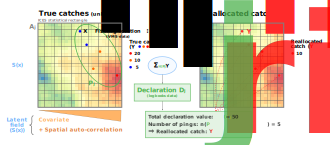
\includegraphics[width=11cm]{images/realloc.png}

\onslide<2-3>{

\begin{table}
  \centering \scriptsize
  \begin{tabular}{ M{2cm} M{4cm} M{4cm} }
  \textcolor{BaptisteRed}{\textbf{Current situation}} & 
  $Y_i | \textcolor{BaptisteBlue}{S}(x_i), x_i \sim \mathcal{L}_Y(\textcolor{BaptisteBlue}{S}(x_i),\xi,\sigma^2)$          &
  $Y_i=\frac{\textcolor{BaptisteLightGreen}{D_j}}{ \operatorname{n}(\textcolor{BaptisteLightGreen}{\mathcal{P}_j})}=\textcolor{BaptisteRed}{Y_i^*}$ \\
  \end{tabular}
\end{table}

}

\onslide<3>{

\begin{table}
  \centering \scriptsize
  \begin{tabular}{ M{2cm} M{2cm} M{4cm} M{2cm} }
  \textcolor{BaptisteLightGreen}{\textbf{Alternative solution}} & 
  $\textcolor{BaptisteLightGreen}{D_j}=\sum_{\textcolor{BaptisteLightGreen}{i \in \mathcal{P}_j}}{Y_{i}}$          &
  $\textcolor{BaptisteLightGreen}{D_j} | \textcolor{BaptisteBlue}{S}_{\textcolor{BaptisteLightGreen}{\mathcal{P}_j}},\textcolor{BaptisteLightGreen}{\mathcal{P}_j} \sim \mathcal{L}_D( \textcolor{BaptisteBlue}{S}_{\textcolor{BaptisteLightGreen}{\mathcal{P}_j}},\xi,\sigma^2)$
  & \textcolor{BaptisteBlue}{\ding{224}}  Match $\mathcal{L}_D$ and $\mathcal{L}_Y$ moments \\ 
  \end{tabular}
\end{table}

}

\end{frame}

\begin{frame}{Two alternative procedures to reallocate catches}
\protect\hypertarget{two-alternative-procedures-to-reallocate-catches-1}{}

\textbf{Punctual observation model} (\(Y_i\))

\scriptsize \(\operatorname{L}(y,\mu,\sigma^2)\) is the lognormal
likelihood for observation \(y\), mean \(\mu\) and variance \(\sigma^2\)

\(Y\) and \(D\) are supposed conditional on S and x \footnotesize

\[
\operatorname{P}\left(Y_i=y_{i} \right) =
\left\{
    \begin{array}{ll}
        p_i & \text { if } y_{i}=0 \\
        \left(1-p_i\right) \cdot \operatorname{L}\left(y_{i },\mu_i=\frac{S(x_i)}{\left(1 - p_i\right)},\sigma^{2} \right) & \text { if } y_{i} > 0
    \end{array}
\right.
\]

\[p_{i}=\exp(-e^\xi .S(x_{i}))\]

\normalsize \vspace{\baselineskip} \vspace{\baselineskip}

\onslide<2>{

\textcolor{BaptisteLightGreen}{\textbf{Declaration model}} ($D_j=\sum_{i \in \mathcal{P}_j}{Y_{i}}$)

\footnotesize

\begin{align*}
P(D_j = 0) & = \prod_{i\in \mathcal{P}_j} P(Y_{i} = 0)
                      = \exp{ \left \lbrace- \sum_{i\in \mathcal{P}_j} e^{\xi}. S(x_{i})\right \rbrace} = \pi_j
\end{align*}

\normalsize \vspace{\baselineskip}

$$\operatorname{P}\left(D_j=d_{j} \vert d_j > 0 \right) = \quad \textcolor{red}{\textbf{?}}$$

}

\end{frame}

\begin{frame}{Specifying
\(\operatorname{P}\left(D_j=d_{j} \vert d_j > 0 \right)\)}
\protect\hypertarget{specifying-operatornamepleftd_jd_j-vert-d_j-0-right}{}

\normalsize

\textbf{Compute the moments of $\mathbf{D_j\vert d_j > 0}$}

\footnotesize

\[E(D_j \vert d_j > 0)=\frac{\sum_{i \in \mathcal{P}_j} S(x_{i})}{1-\pi_j}\]

\[Var(D_j \vert d_j > 0) = \frac{\sum_{i \in \mathcal{P}_j} Var(Y_{i})}{1-\pi_j} - \frac{\pi_j}{(1-\pi_j)^2}E(D_j)^2\]

\[Var(Y_{i})=\frac{S(x_{i})^2}{1-p_{i}}(e^{\sigma^2}-(1-p_{i}))\]

\vspace{\baselineskip}
\vspace{\baselineskip}

\normalsize

\onslide<2>{

\textbf{Consider $\mathbf{D_j\vert d_j>0}$ is Lognormal too}

\footnotesize

\vspace{\baselineskip}

$$
\begin{aligned}
&\operatorname{P}\left(D_j=d_{j} \vert d_j > 0 \right) = \\ \\ & \quad \quad \operatorname{L}\left(d_{j},\mu_j = E(D_j|d_j>0),\sigma_j^2 = ln(\frac{Var(D_j|d_j>0)}{E(D_j|d_j>0)^2} + 1) \right)
\end{aligned}
$$

}

\end{frame}

\begin{frame}{Simulation-estimation and case study}
\protect\hypertarget{simulation-estimation-and-case-study}{}

\begin{columns}
\begin{column}{0.5\textwidth}

\center
\textbf{Simulation-estimation}

\end{column}
\begin{column}{0.5\textwidth}

\end{column}
\end{columns}

\tiny \vspace{\baselineskip}

\begin{columns}
\begin{column}{0.5\textwidth}


\begin{columns}
\begin{column}{0.45\textwidth}

\includegraphics[width=3cm]{images/data_plot.png}

\end{column}
\begin{column}{0.55\textwidth}
\footnotesize
\textbf{Simulation}
\tiny
\begin{itemize}
\item \scriptsize \textcolor{BaptisteBlue}{\textbf{Latent field}} \tiny (\textcolor{BaptisteOrange}{covariate} + \textcolor{BaptisteBrown}{spatial random effect})
\item \scriptsize \textbf{Commercial data} \tiny (3000 samples over 2/3 of the area)
\item \scriptsize \textcolor{BaptisteLightGreen}{\textbf{Reallocation process}} \tiny (10 locations per declaration)
\item \scriptsize \textcolor{SurveyBlue}{\textbf{Scientific data}} \tiny (100 samples over the whole the area)
\end{itemize}

\end{column}
\end{columns}

\scriptsize
\vspace{\baselineskip}

\onslide<2-4>{
\footnotesize
\textbf{Estimation} \scriptsize \\
Comparison of 3 model configurations: \\
\tiny \vspace{\baselineskip} \scriptsize
1/ Model fitted to \textbf{\textcolor{SurveyBlue}{scientific data}} only \\
\tiny \vspace{\baselineskip} \scriptsize
2/ \textcolor{BaptisteDarkGrey}{\textbf{Integrated model}} (= \textbf{\textcolor{SurveyBlue}{scientific}} + \textbf{commercial data}) with \textcolor{BaptisteRed}{commercial likelihood built on $\bf{Y_i^*}$} \\
\tiny \vspace{\baselineskip} \scriptsize
3/ \textcolor{BaptisteDarkGrey}{\textbf{Integrated model}} with \textcolor{BaptisteLightGreen}{commercial likelihood built on $\bf{D_j}$} \\
\tiny \vspace{\baselineskip}

Estimation realized through TMB (Template Model Builder) \\
100 runs of simulation-estimation

}

\end{column}
\begin{column}{0.5\textwidth}

\onslide<3-4>{

\footnotesize
\textbf{Model evaluation} \scriptsize \\
1/ Mean square prediction error \\
$$MSPE=\frac{\sum_{x=1}^n (\textcolor{BaptisteBlue}{S(x)} - \textcolor{BaptisteBlue}{\hat{S}(x)} ) ^2}{n}$$

\vspace{\baselineskip}

2/ Covariate effect (or species-habitat relationship): \\
$$\textcolor{BaptisteOrange}{\beta_S} = 2 \, \, \, \text{versus} \, \, \, \textcolor{BaptisteOrange}{\hat{\beta}_S}$$
\vspace{\baselineskip}

}

\onslide<4>{

\normalsize
\begin{center}
\textbf{Case study:} \scriptsize Sole in the Bay of Biscay \\
\end{center}

\begin{columns}
\begin{column}{0.5\textwidth}
\center
\includegraphics[width=2cm]{images/solea_solea.png}
\vspace{\baselineskip}
\vspace{\baselineskip}
\end{column}
\begin{column}{0.5\textwidth}
\tiny \textcolor{SurveyBlue}{\textbf{Survey data:}} Orhago\\
\textbf{Commercial data:} OTB-DEF trawlers (to ease convergence onboard observer data were integrated in the fit)\\
\textbf{Fitted models:} same as simulations\\
\textcolor{BaptisteOrange}{\textbf{Covariate:}} substrate

\normalsize \vspace{\baselineskip}
 
\end{column}
\end{columns}

}

\end{column}
\end{columns}

\end{frame}

\hypertarget{results}{%
\section{Results}\label{results}}

\begin{frame}{Simulation-estimation}
\protect\hypertarget{simulation-estimation}{}

\center

\begin{columns}
\begin{column}{0.4\textwidth}

\center
\includegraphics[width=4cm]{images/res_simu_plot.png}

\end{column}

\begin{column}{0.6\textwidth}
\center

\includegraphics[width=5.5cm]{images/map_simu_plot.png}
\vspace{\baselineskip}

\end{column}

\end{columns}

\end{frame}

\begin{frame}{Case study: Sole in the Bay of Biscay}
\protect\hypertarget{case-study-sole-in-the-bay-of-biscay}{}

\center

\begin{columns}
\begin{column}{0.4\textwidth}

\begin{center}
\includegraphics[width=4.5cm]{images/par_plot.png}
\end{center}
\scriptsize
\onslide<2>{

The \textcolor{BaptisteDarkGrey}{\textbf{integrated model}} fitted to \textcolor{BaptisteLightGreen}{$\bf{D_j}$}:

\textbf{\textcolor{BaptisteBlue}{\ding{224}}} Recovers the species-habitat relationship ($\bf{\textcolor{BaptisteOrange}{\beta_S}}$)

\textbf{\textcolor{BaptisteBlue}{\ding{224}}} Modifies the \textbf{contrasts of the map} \tiny (shape and intensity of the hotspots/coldspots) \scriptsize

}

\end{column}

\begin{column}{0.6\textwidth}
\center
\includegraphics[width=5.5cm]{images/case_study_plot.png}
\vspace{\baselineskip}

\end{column}

\end{columns}

\end{frame}

\hypertarget{discussion}{%
\section{Discussion}\label{discussion}}

\begin{frame}{Discussion}
\protect\hypertarget{discussion-1}{}

\begin{itemize}

\item \textcolor{BaptisteDarkGrey}{\textbf{Integrated framework}} that combines \textcolor{BaptisteLightGreen}{\textbf{catch declarations data}} (rough resolution) and \textcolor{SurveyBlue}{\textbf{scientific data}} (exact locations) \\
\textcolor{BaptisteBlue}{\ding{224}} Allows to estimate the \textcolor{BaptisteOrange}{\textbf{habitat effect}} through commercial data \\
\textcolor{BaptisteBlue}{\ding{224}} Modifies the \textbf{contrasts of the map} (hotspots vs. coldspots)

\tiny \vspace{\baselineskip} \normalsize

\onslide<2-4>{

\item \textbf{Some limits:}

\textcolor{BaptisteBlue}{\ding{224}} How to ease convergence ? \\

\textbf{\textcolor{BaptisteBlue}{\ding{224}}} Need to make the hypothesis that fishing locations ($\textcolor{BaptisteLightGreen}{\mathcal{P}_j}$) are known

}

\tiny \vspace{\baselineskip} \normalsize

\onslide<3-4>{

\item \textbf{Is it a generic framework ?} \\

\textbf{\textcolor{BaptisteBlue}{\ding{224}}} The overall approach is, \scriptsize \\ \textit{(i.e. modelling observed aggregated observations as a sum of latent punctual observations)}

\normalsize \textbf{\textcolor{BaptisteBlue}{\ding{224}}} But need to adapt the observation model to the data \scriptsize \\ \textit{(here zeroinflated positive continuous data)}

}

\tiny \vspace{\baselineskip} \normalsize
 
\onslide<4>{

\item \textbf{Moving to space-time ?} \\

\textbf{\textcolor{BaptisteBlue}{\ding{224}}} Extending the observation model to account for \textbf{temporal misalignment} \\

\textbf{\textcolor{BaptisteBlue}{\ding{224}}} Including spatio-\textbf{temporal covariance} in the latent field \\

}


\end{itemize}

\end{frame}

\hypertarget{section}{%
\section{}\label{section}}

\begin{frame}{}

\tiny \vspace{\baselineskip}

\centering \Large \textcolor{BaptisteGrey}{\textbf{Thank you for your attention!}}

\tiny \vspace{\baselineskip}

\begin{figure}
    \includegraphics[width=11cm]{images/front_page.png}
\end{figure}

\end{frame}

\end{document}
